\section{Metropolis-Hastings MCMC (nonlinear model)}

The data for this problem can be described by a Gaussian function given by,
\begin{equation}
    f(\Vec{x}|\Vec{a})=a_0+a_1e^{-\frac{1}{2}(\frac{x-a_2}{a_3})^2}.
    \label{eq:GaussModel}
\end{equation}
where our parameters $a_0,a_1,a_2,a_3$ represent an offset, amplitude, center and width of the Gaussian being modeled.

We fit our model to the data by using \emph{curve\_fit} from \emph{scipy.optimize} in Python by implementing an LM \\method.
From this, we obtained our best fit parameters and a covariance matrix. 

Using the Metropolis-Hastings method described in the previous exercise and the best fit parameters, we can determine the joint posterior probability distribution as well as the marginalized posterior probability. 
These are shown in Figure \ref{fig:GaussHastings} with the contours representing the 68.3\% and 95\% confidence intervals for all combinations of parameters.

Note that the histograms shows that our parameters have a marginalized posterior probability similar to a normal distribution. 

Looking at the joint probability we can note that \\the offset,$a_0$, and the amplitude, $a_1$, are uncorrela-ted with the center,$a_2$, of the Gaussian model. 
This makes sense since the center location wouldn't affect the overall shape of the Gaussian. We can also note that the width, $a_3$, is lightly correlated to the rest of the parameters.
Additionally, the amplitude and the offset are also lightly correlated with each other. 

% Use the same Metropolis Hastings code to fit the data from gaussfit data.npz to the gaussian function
% \begin{equation}
%     f(\Vec{x}|\Vec{a})=a_0+a_1e^{-\frac{1}{2}(\frac{x-a_2}{a_3})^2}
% \end{equation}
% Overplot the joint 68.3\% and 95\% confidence intervals for all combinations of parameters.

\begin{figure*}
    \centering
    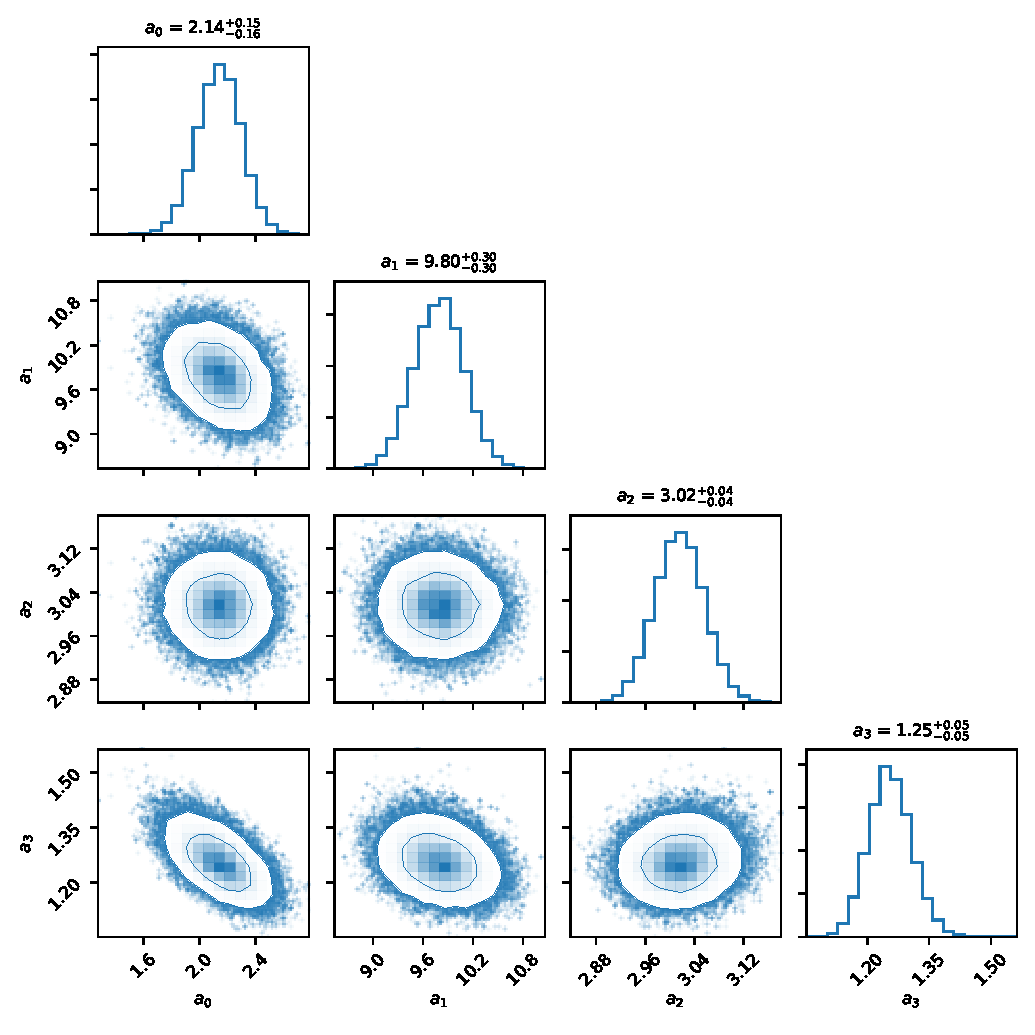
\includegraphics{CodeAndFigures/GaussianModelMetropolisHastings.pdf}
    \caption{Joint posterior probability distribution as well as the marginalized posterior probability of the data using the model described in equation \ref{eq:GaussModel}. The contours show the 68.3\% and 95\% confidence intervals.}
    \label{fig:GaussHastings}
\end{figure*}